\documentclass{tufte-handout}
\usepackage{amsmath,amsthm}

\input{vc.tex}

\usepackage{pgfplots}
\pgfplotsset{width=\textwidth,compat=1.5.1}

\newtheorem{claim}{Claim}[section]
\title{\sf Approximation Algorithm for Maximum Cut}
%\date{\GITAuthorDate}
%\author{Thore Husfeldt}

\begin{document}
\maketitle
\footnotetext{rev. \GITAbrHash}

\section{Maximum Cut}
Consider an undirected graph $G=(V,E)$ with positive edge weights
$w(e)$ $(e\in E)$.
Set $n=|V|$ and $m=|E|$.
The Maximum Cut problem (Maxcut) is to find a partition of the
vertices with the largest total weight of the edges ``crossing'' the
partition, i.e., maximising the value of \[c(A)= \sum_{(u,v)\in E,
  u\in A, v\notin A} w(u,v)\,\] over all $A\subseteq V$.

Maxcut is NP-hard, so we have little hope of writing an algorithm that
solves arbitrary Maxcut instances optimally.

\subsection{Algorithm R}

Consider the following simple randomized algorithm (call it
Algorithm~R): Let $A$ be a \emph{random subset} of $V$ constructed by
flipping a coin $r(v)\in\{0,1\}$ for every vertex $v\in V$ and setting
$v\in A$ if and only if $r(v)=1$.

\subsection{Inputs}

The  data directory contains two input instances:
\begin{description}
\item[ pw09\_100.9.txt:] A random instance with $|V|=100$ and
  $|E|=4455$. The best cut in this instance is
  13659.\sidenote{A. Wiegele, Biq Mac Library - A collection of Max-Cut
    and quadratic 0-1 programming instances of medium size, 2007.}
\item[ matching\_1000.txt:] A disjoint union of 500 edges with unit weight.
\end{description}

The input format is straightforward: the first line contains $n$ and
$m$; every following line describes an edge in the format first
vertex, second vertex, weight.
All weights are integers, vertices are numbered $1,2,\ldots, n$.

\subsection{Deliverables}

\begin{enumerate}
\item Implement algorithm R and run it on the dataset provided in
  the data directory.
  Use whatever programming language and libraries you want, but make
  sure that your code is short and crisp; my own solution takes 25
  lines.
  Attach a printout to the report or have it checked by your lab
  assistant.
\item Fill out the report on the next page; you can just use the
  \LaTeX\ code if you want.
\end{enumerate}

\newpage


\newpage
\section{Maxcut Lab Report}


by Oscar Olsson and Tommy Ivarsson.

\subsection{Running time}

The running time of algorithm~R is $O(n + m)$.

\subsection{Randomness}

Algorithm R uses $n$\sidenote{Replace
  $[\ldots]$ by a function of $n$ and/or $m$. Do not use asymptotic
  notation. This is supposed to be easy.} random bits.

\subsection{Solution quality}

\paragraph{Experiments.}

\begin{enumerate}
\item
For the input file  pw09\_100.9.txt with $t=100$ runs, we found
an average cutsize of $C=12343$, roughly $90.3$\% of the optimum
$\operatorname{OPT} = 13659$.
The distribution of cutsizes looks as follows:

\medskip

\noindent
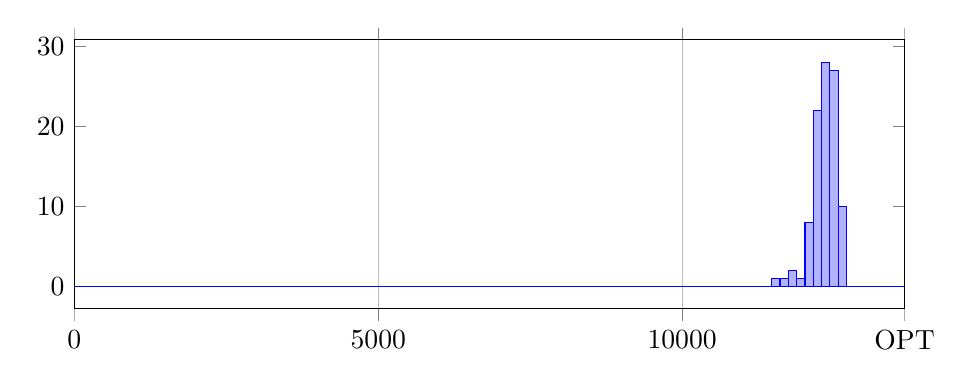
\begin{tikzpicture}
\begin{axis}[
  height= 5cm,
  ybar interval,
  xmin = 0,  xmax = 13659,
  xtick =       {0   ,   5000,   10000, 13659},
  xticklabels = {$0$, $5000$, $10000$,   OPT},
  x tick label as interval = false,
  scaled ticks = false
]
    \addplot+[hist={bins=100}]
        table[y index=0] {% output of 
          % perl -e "for $i (1..100) { system 'python sol/rmaxcut.py < data/pw09_100.9.txt '}"
%\input{../MCR_res.tex}
%\input{thore_res.txt}
12455
12488
12294
12460
12255
12177
12523
11532
12244
12442
12194
12544
12414
12530
12175
12154
12535
12383
12504
12535
12221
12617
12446
12148
12430
12463
12386
12251
12042
12329
11985
12237
12250
12401
12160
12542
12309
12353
12463
12567
12373
12359
12480
12658
12418
12382
12332
12284
12690
12158
12589
11843
12365
12287
12293
12430
12224
12519
12099
11832
12470
12660
12513
12423
12225
12275
12395
12169
12384
12513
12575
12326
12278
12368
12518
12420
12302
12587
12324
12308
12065
12476
12414
12473
12480
12570
12229
12132
11733
12390
12144
12353
12308
12234
12028
12631
12216
12472
12429
12526
    };
\end{axis}
\end{tikzpicture}

\item
For the input file matching\_1000.txt with $t=100$ runs, we found an average
cutsize of $C=250$, roughly $50$\% of the optimum $\operatorname{OPT} = 500$.

The optimum was derived by alanyzing the input. The input consists of $500$
pairs of vertices, each pair is connected by one edge of weight $1$. There are
no edges between any of the pairs. By choosing one, and only one, vertex from
each pair the maxcut becomes $500$, $500$ pairs and in each pair the edge is
part of the cut, which is also the sum of all edges and the optimum result.

The distribution of cutsizes looks as follows:

\medskip

\noindent
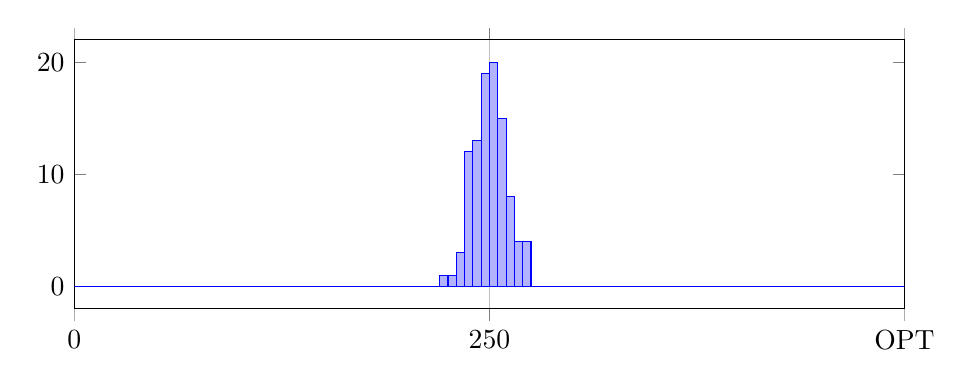
\begin{tikzpicture}
\begin{axis}[
  height= 5cm,
  ybar interval,
  xmin = 0,  xmax = 500,
  xtick =       {0   ,   250,   500},
  xticklabels = {$0$, $250$,   OPT},
  x tick label as interval = false,
  scaled ticks = false
]
    \addplot+[hist={bins=100}]
        table[y index=0] {% output of 
          % perl -e "for $i (1..100) { system 'python sol/rmaxcut.py < data/pw09_100.9.txt '}"
%\input{../MCR_res.tex}
%\input{thore_res.txt}
243
267
253
247
236
240
248
248
249
252
253
237
252
236
248
237
246
242
252
245
230
241
265
250
254
250
236
252
237
239
241
255
246
253
253
261
263
261
259
257
250
263
257
234
247
250
270
243
254
258
239
262
249
255
235
271
248
224
248
242
245
263
253
249
241
244
236
255
270
241
263
245
259
237
251
236
256
256
265
257
259
249
244
262
257
225
245
252
242
241
249
253
265
234
259
255
271
248
252
251
    };
\end{axis}
\end{tikzpicture}
\end{enumerate}

\paragraph{Analysis of performance guarantee}

Clearly, Algorithm R performs quite badly on input 
  matching\_1000.txt.
We will show that it can perform \emph{no worse} than that, i.e., we
will establish that in expectation, the cutsize $C$ satisfies $C \geq
\frac{1}{2}\cdot \operatorname{OPT}$.\sidenote{Replace [\ldots] by the
  right constant}


We will view $C$ as a random variable that gives the size of the cut
defined by the random choices.
Let $W$ denote the total weight of the edges of $G$, i.e.,
\[ W= \sum_{e\in E} w(e)\,.\]

Then,
\begin{equation}
E[C] = \textstyle\frac{1}{2}\cdot W\,.
\end{equation}

To see this, define the indicator random variable $X_{uv}$ for every
edge $uv\in E$ as follows.
Set $X_{uv}=1$ if $uv$ crosses the cut, i.e., $u\in A$ and $v\notin A$
or $u\notin A$ and $v\in A$.
Otherwise, $X_{uv} = 0$.

Then, $\Pr(X_{uv} = 1) = \Pr(u \in A) \cdots \Pr(v \notin A) + \Pr(u \notin A) \cdot Pr(v \in A) = \frac{1}{2} \cdot \frac{1}{2} + \frac{1}{2} \cdot \frac{1}{2} = \frac{1}{2}$.
Now, $E[C]=[\ldots]$ Finally, we have 
\(E[C]\geq [\ldots]\cdot \text{OPT}\) because clearly
$[\ldots]$.\sidenote{Fill in the missing blanks in this paragraph.
  Your calculations and arguments need to include phrases like
  ``because BLA and BLA are independent'' or ``disjoint,'' and ``by
  linearity of expectation'' and ``because the weights are positive.''

}


\newpage
\section{Optional: Derandomising Algorithm R}

\subsection{Algorithm L} 


We now reduce the number of random bits used by the algorithm to $\log
n$ using a simple \emph{pseudorandom generator}.


Let $k=\lceil\log (n+1)\rceil$ and flip $k$ coins $b_1,\ldots, b_k$.
There are $2^k -1 \geq n$ different ways of choosing a nonempty subset
$S\subseteq [k]$ of the coins.
Each of these ways defines a random bit $r_S =\bigoplus_{i\in S} b_i$.
This gives a total of $n$ random bits.
These random bits are not as high-quality as the original $k$ bits,
but they retain the crucial property of \emph{pairwise independence}:
If $S\neq T$ then 
\[ \Pr(r_S\neq r_T) = [\ldots],.\]

Extend Algorithm~R using this idea; call the resulting
algorithm~L (for logarithmic randomness).

\subsection{Algorithm Z}

For our final trick, we let the random bits disappear completely:
since Algorithm~L uses only $k$ bits of randomness, we can iterate
over \emph{all} coin flips---there are only $2^k$, which is polynomial
(in fact, linear) in $n$.
Extend algorithm~L using this idea; call the resulting algorithm~Z
(for zero randomness).
The running time of Z is $O([\ldots])$.

\newpage
\section{Perspective}

This lab establishes minimal skills in algorithms implementation,
probabilistic analysis of algorithms (independence, linearity of
expectation, and in particular the trick of computing an expectation
using indicator random variables), and approximation guarantees (in
particular, finding upper and lower bounds by exhibiting a concrete
``bad instance'' and a comparison to a hypothetical optimum,
respectively).
The histogram aims to establish the intuition that measure is
concentrated around its expectation.

\bigskip

To establish that Maxcut is NP-hard one reduces from NAE-Sat, a
reduction that can be found in many places\sidenote{C. Moore and
S. Mertens, \emph{The Nature of Computation}, Oxford University Press,
  2011, p. 146.}
Recall that the related problem \emph{Minimum Cut} is easy because of
the max flow--min cut theorem.
A moment's thought should convince you that as soon as negative
weights are allowed, the two problems are the same (and both are
hard).
Algorithm R doesn't work at all for negative weights.

Algorithm R is a classical randomised approximation algorithm, its
origins seem to be shrouded in the mists of time.
The \emph{deterministic} algorithm of Sahni and Gonzales\sidenote{S.\
  Sahni and T.\ Gonzalez.
  P-complete approximation problems.
  \emph{J.\ Assoc.\ Comput.\ Mach.}, 23(3):555--565, 1976.}
can be viewed as a derandomisation of R using the \emph{method of
  conditional expectations}.
These algorithms were best knows until the breakthrough result of
Goemans and Williamson,\sidenote{M.\ X.\ Goemans and D.\ P.\
  Williamson.
  Improved approximation algorithms for maximum cut and satisfiability
  problems using semidefinite programming.
  \emph{J.\ Assoc.\ Comput.\ Mach.}, 42(6):1115--1145, 1995.}
which improved the approximation factor to $0.87856$.
H\aa{}stad has shown that no algorithm can approximate the maxcut
better than $16/17\sim 0.941176$ unless P equals NP\@. Khot has shown
that the Goemans--Williamson bound is essentially optimal under the
\emph{Unique Games Conjecture}.

Algorithm L can also be viewed as an application of \emph{pairwise
  independent hash functions}.


\end{document}
